%-------------------------------------------------------------------------------
\section{Eval}
\label{s:eval}
%-------------------------------------------------------------------------------

In our evaluation, we explore the following questions:
\begin{enumerate}
    \item Does the patch isolate LC from BE workloads for real applications?
    \item How much does the patch cost?
\end{enumerate}

All the graphs in this paper run on Linux version 6.14.2, the baseline version
that our patch builds on.

\subsection{Realistic applications}


\begin{figure}[t]
    \centering
    \begin{subfigure}[t]{0.49\columnwidth}
        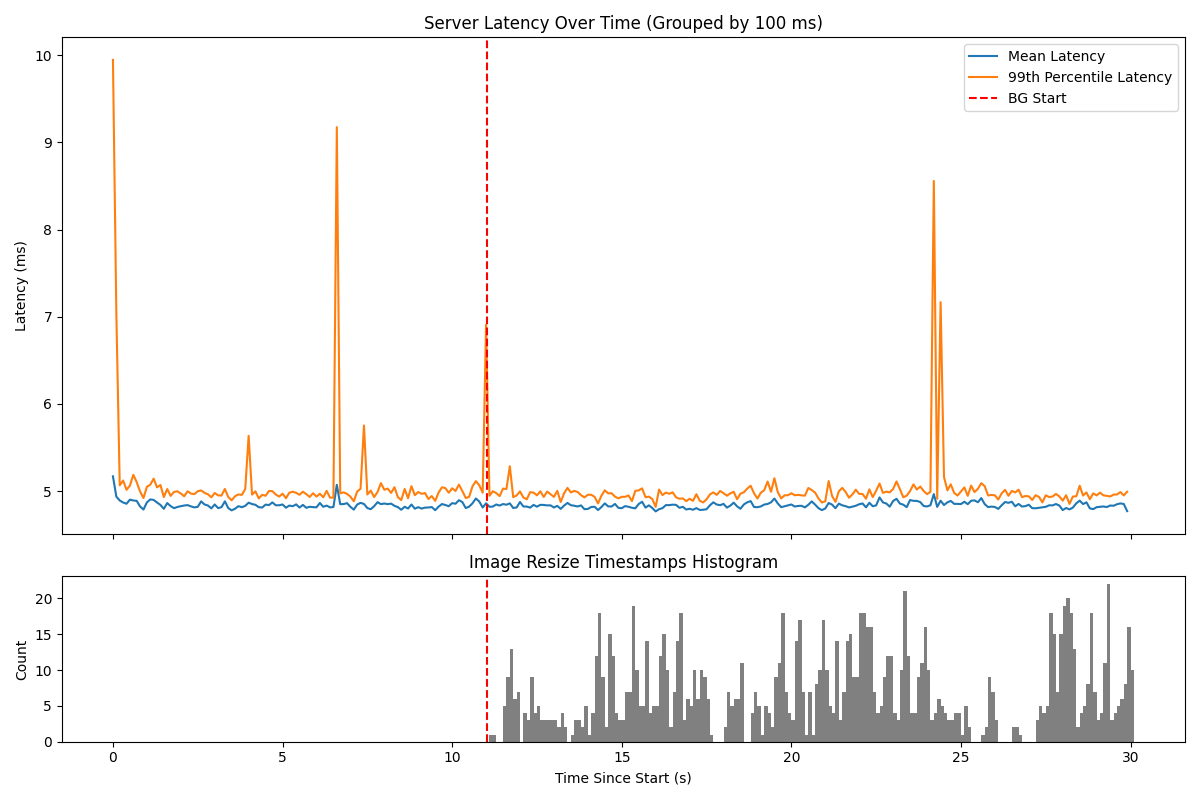
\includegraphics[width=\columnwidth]{graphs/patched-idle-low-two.png}
        \caption{Low load}\label{fig:patched-idle-low-two}
    \end{subfigure}
    \hspace{\fill}
    \begin{subfigure}[t]{0.49\columnwidth}
        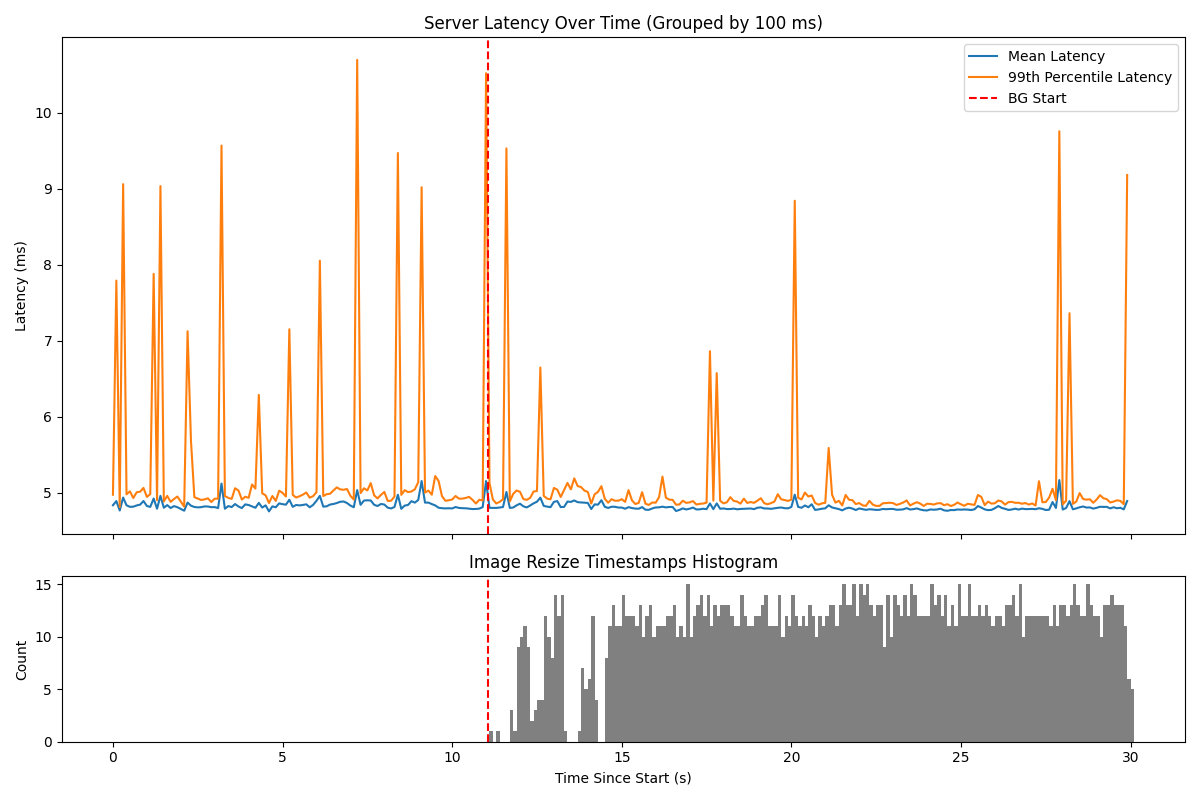
\includegraphics[width=\columnwidth]{graphs/patched-idle-high-two.png}
        \caption{High load}\label{fig:patched-idle-high-two}
    \end{subfigure}
    \vspace{4pt}
    \caption{using a patched \schedidle{} that steals queued \schednormal{}
    tasks before running \schedidle{} ones}\label{fig:patched-idle}
\end{figure}

\begin{figure}[t]
    \centering
    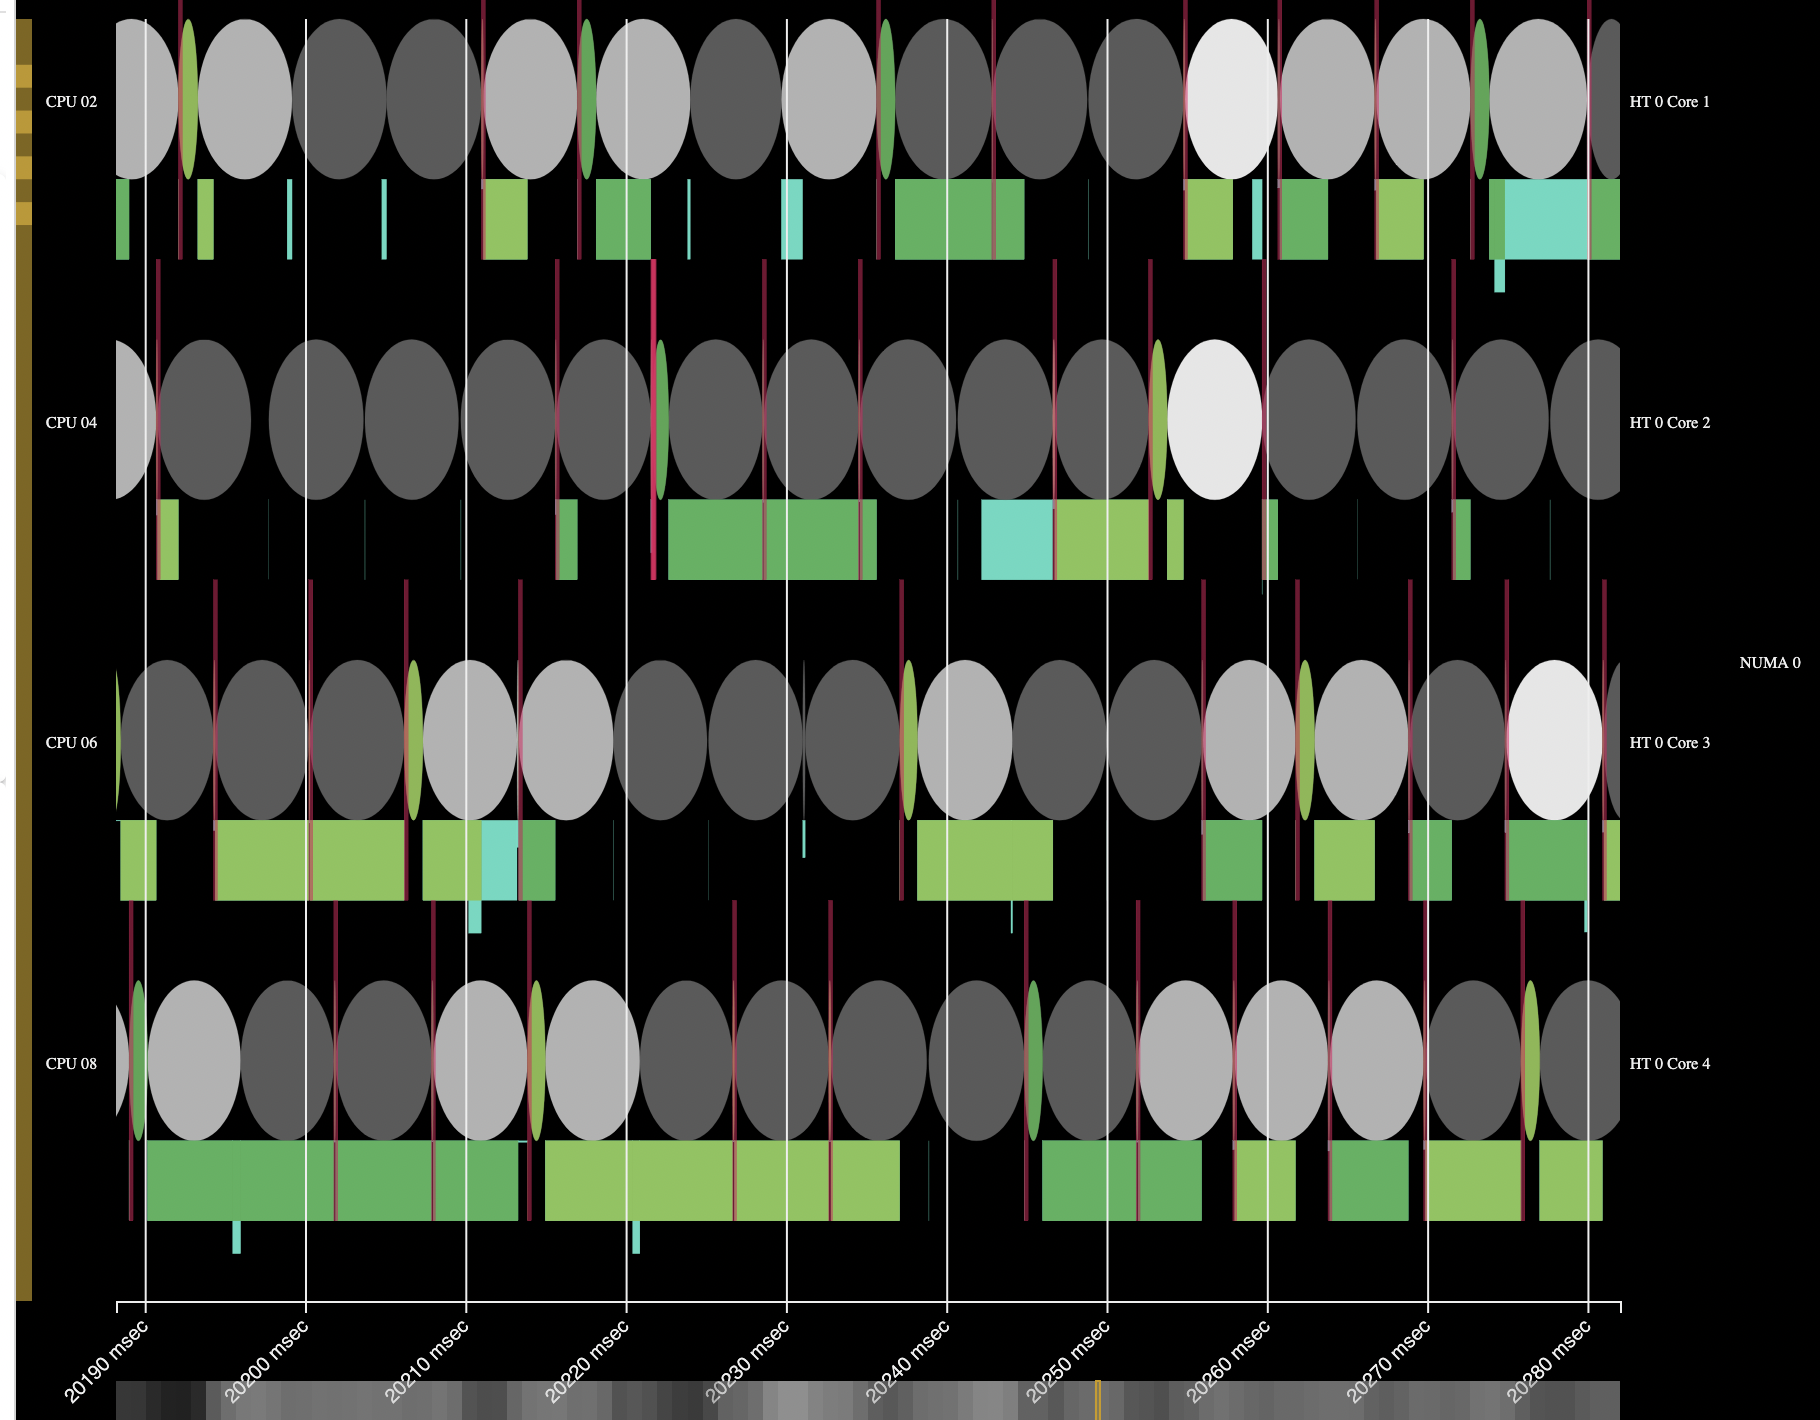
\includegraphics[width=\columnwidth]{graphs/schedviz-patched.png}
    \caption{The BE threads are colored in two different shades of green, the LC
    threads are the grey ones, the red vertical lines are the scheduler
    initially choosing a BE thread, which leads to an attempt to steal a queued
    LC one. As a result, BE threads only run when there are no queued LC
    threads.}\label{fig:schedviz-patched}
\end{figure}

This work focuses on cpu allocation, and thus will show the strongest gains for
applications that are cpu bound. 

We test the patch in two different settings: the cpu-bound example server we
have been using for the graphs in this paper so far, and an example web application
that we run using Kubernetes, that uses a mix of i/o and cpu.

For the experiment we have used throughout the paper, we set the BE workloads to
be marked as idle via the \cgroups{} api. We can see the resulting performance
in \autoref{fig:patched-idle}. As desired the latency of the server remains
stable after the background tasks start. This does not mean that the background
task never runs: the lower graph still shows iterations of image resizing being
done. The difference is that now the background tasks will reliably get
interrupted when the LC server has a request to process. We can see this
happening in an outtake of the schedviz visualization for one of the runs in
\autoref{fig:schedviz-patched}. The green BE processes only run in the gaps
where there is no queued LC process, and are immediately preempted when one
wakes up, on whatever core that may be. The red lines show when the core has
chosen intially to run a BE process, sometimes followed by an LC process that
was stolen as a result running next, sometimes by the BE process actually
running because there was no queued LC thread to steal.

For the web application, we build a REST-api on top of FastAPI, and deploy it
using async gunicorn workers. The web application itself is a recommendation
service, it has a connection to a database, which is makes requests to and
processes data from.



% \subsection{Verifying patch behavior}

% \begin{figure}[t]
%     \centering
%     \begin{subfigure}[t]{0.49\columnwidth}
%         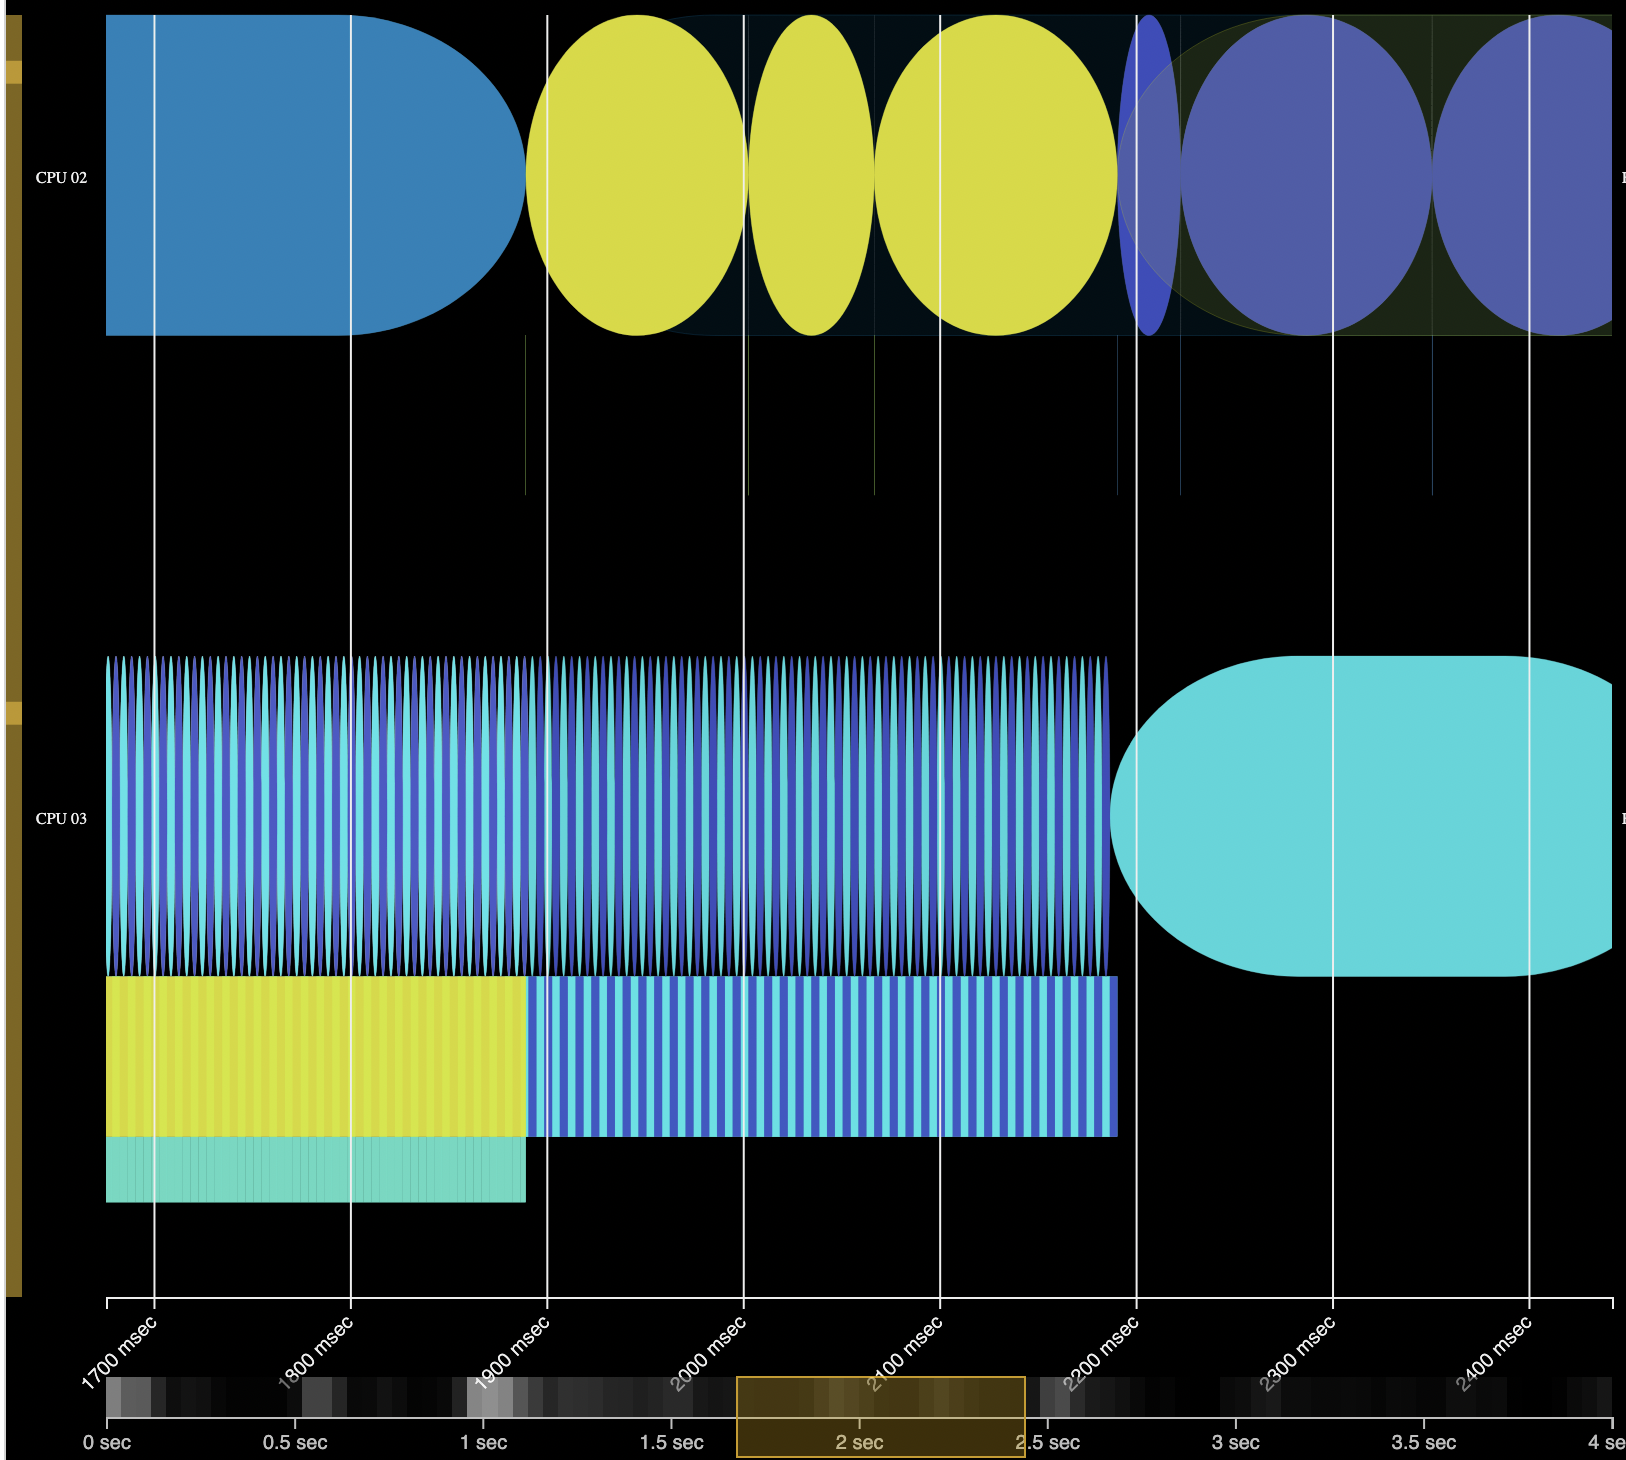
\includegraphics[width=\columnwidth]{graphs/schedviz-steal-unedited.png}
%         \caption{unedited Linux}
%     \end{subfigure}
%     \hspace{\fill}
%     \begin{subfigure}[t]{0.49\columnwidth}
%         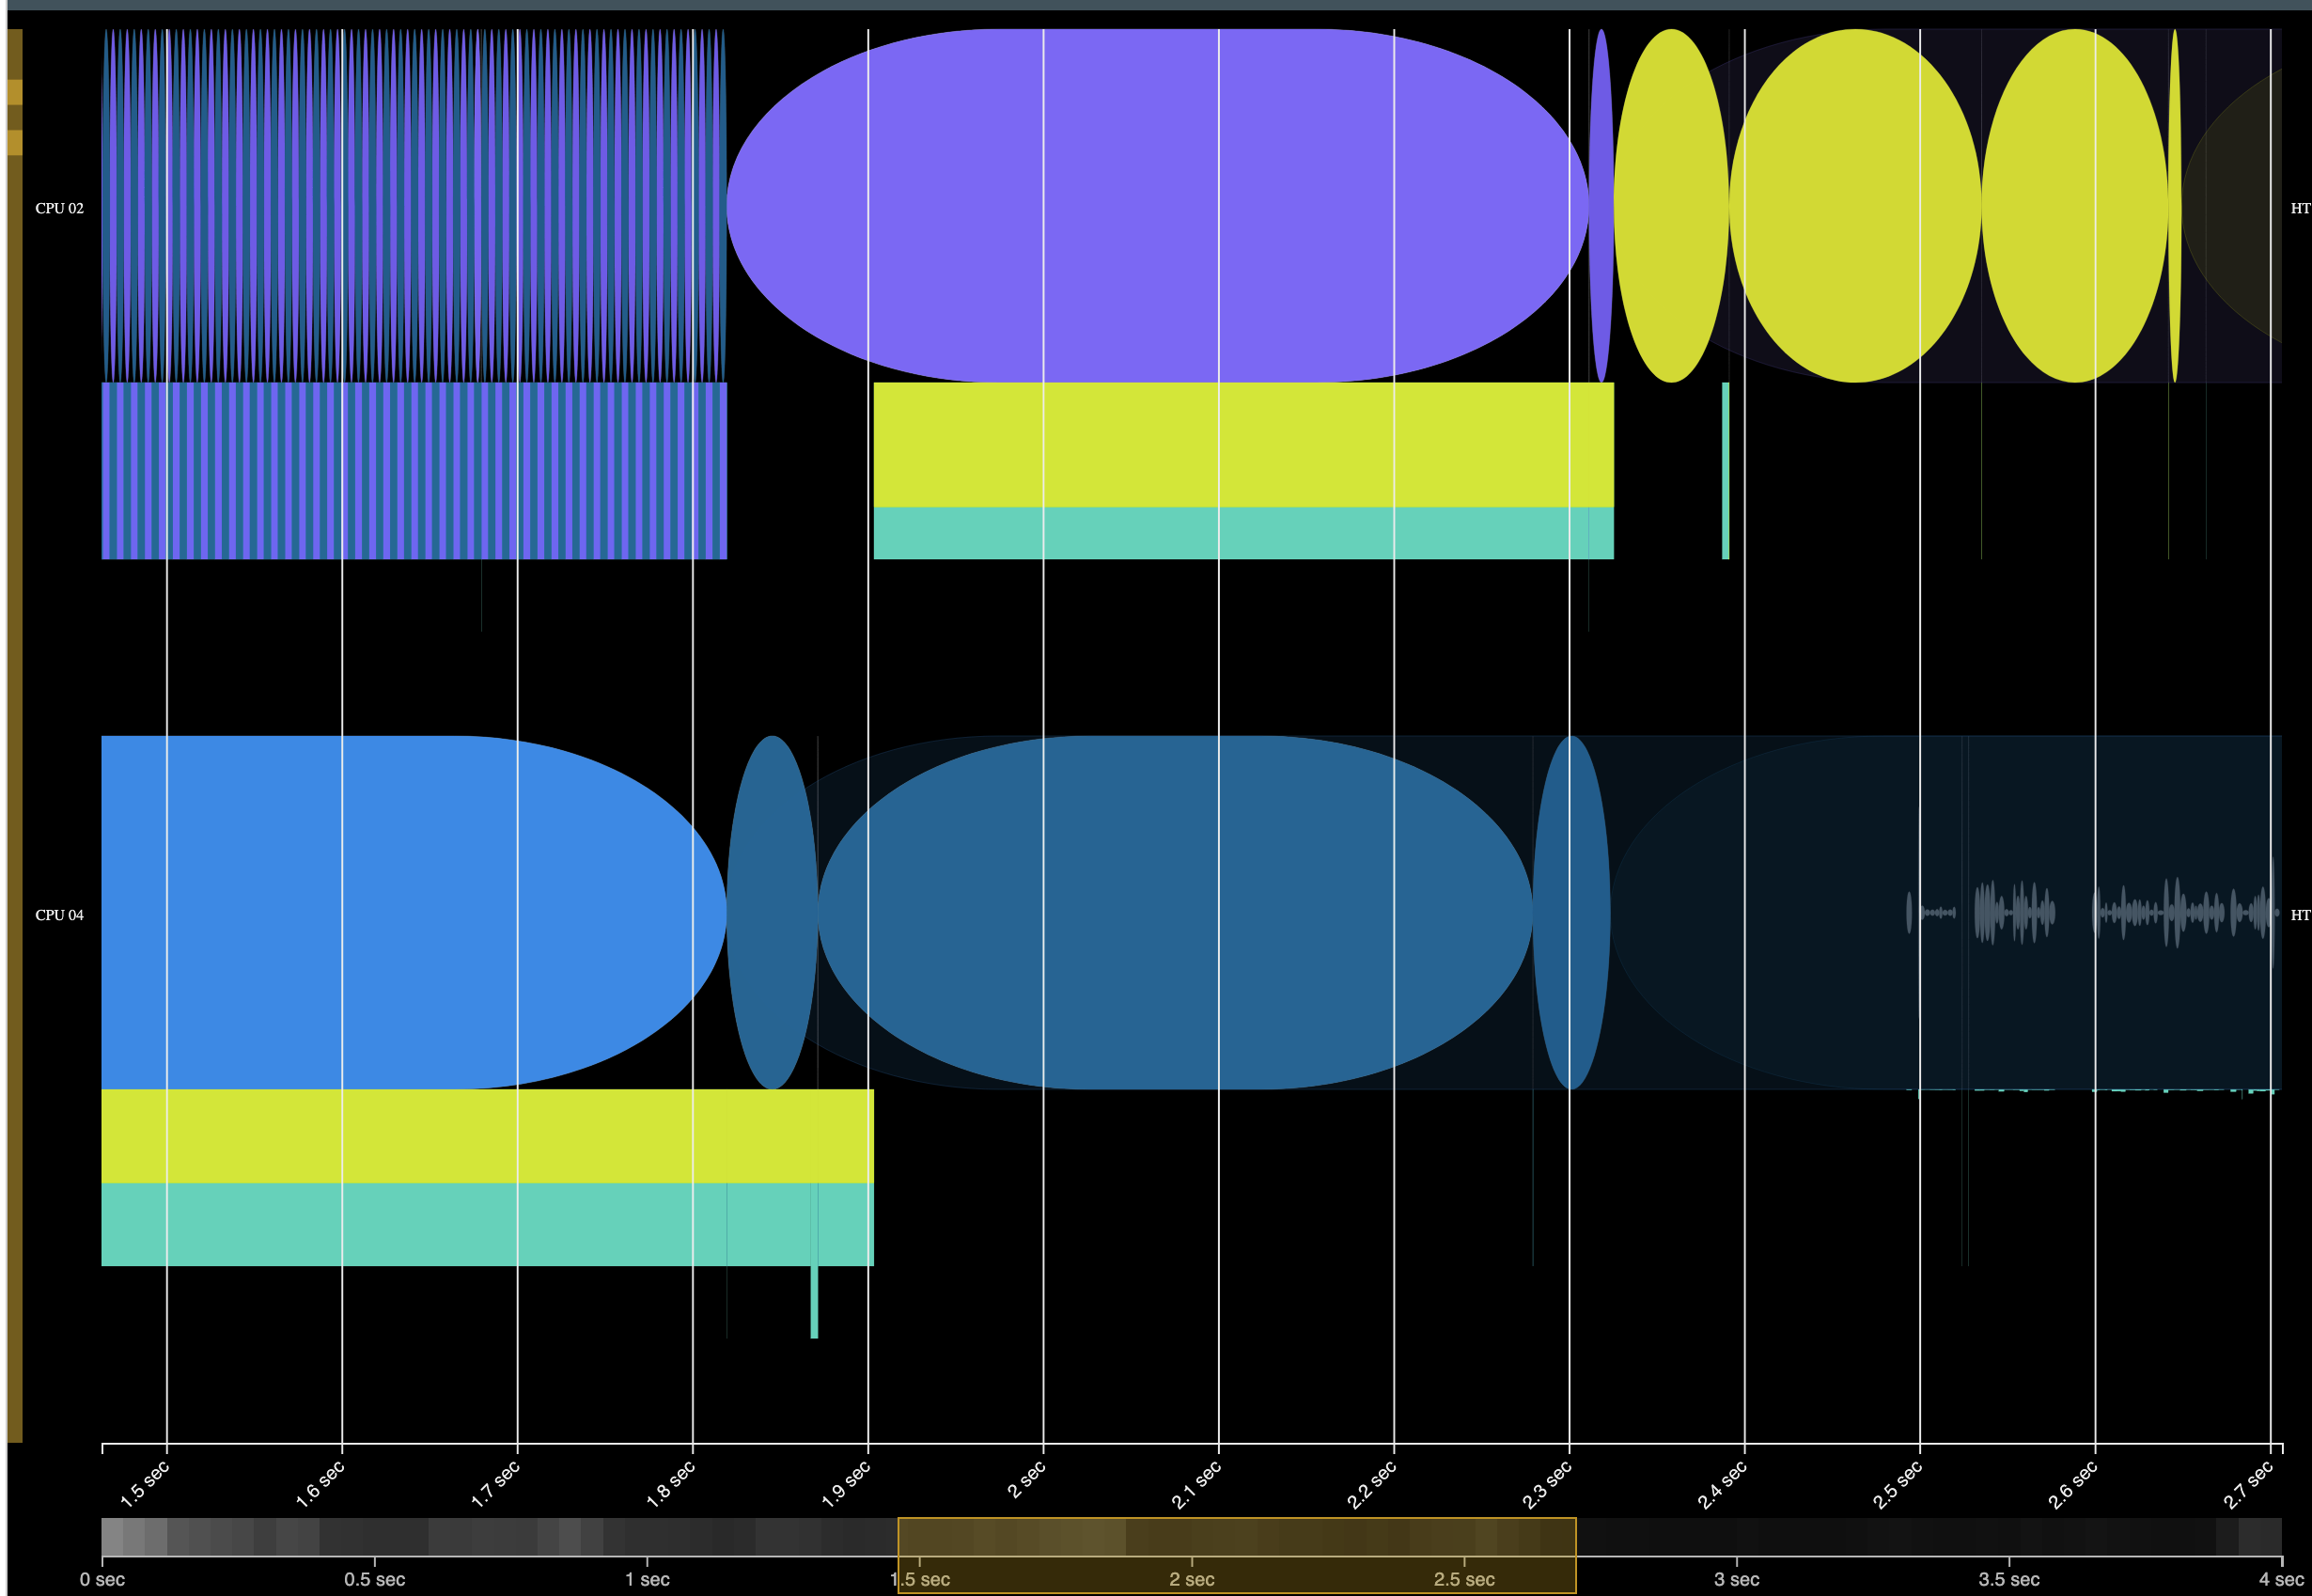
\includegraphics[width=\columnwidth]{graphs/schedviz-steal-patched.png}
%         \caption{patched Linux}
%     \end{subfigure}
%     \vspace{4pt}
%     \caption{microbench on two cores; in both diagrams the different shades of blue are the
%     \schednormal{} processes and the yellow is the \schedidle{} process}\label{fig:steal-micro}
% \end{figure}

% We begin by looking at the behavior of the patch in a microbenchmark. On three
% cores, we run two \schednormal{} processes and one \schedidle{} process. We
% visualize the scheduling decisions made by both an unedited and patched version
% of the kernel in \autoref{fig:steal-micro}. We observe that the scheduler
% initially runs two of the \schednormal{} processes on one core and the third on
% the other core. When the latter finishes, the unedited version of Linux will run
% the \schedidle{} process on that core; whereas the patched version will steal
% the queued \schednormal{} process from the other core. 

% We conclude that the patch works as expected, and is able to enforce the
% categorical separation of \schednormal{}, ie LC, and \schedidle{}, ie BE,
% workloads across cores.